\section{Crowdsourcing addresses: our approach}

\subsection{The social machines mix}

    Although the OLAF data is conceptually simple, assembling such a large dataset while assuring sufficient quality is a complex task, even when starting from such valuable pre-existing open data such as Ordnance Survey's offering.
    
    It is our hypothesis that, to make the best use of pre-existing open data and potentially available technology and human resources, such a problem can be decomposed in a series of complementary sub-problems targeting parts of its scope, each addressed by a dedicated socio-technical system, or social machine. This decomposition can take place over several iterations, hence creating a hierarchy of systems. 

    \begin{figure*}
    	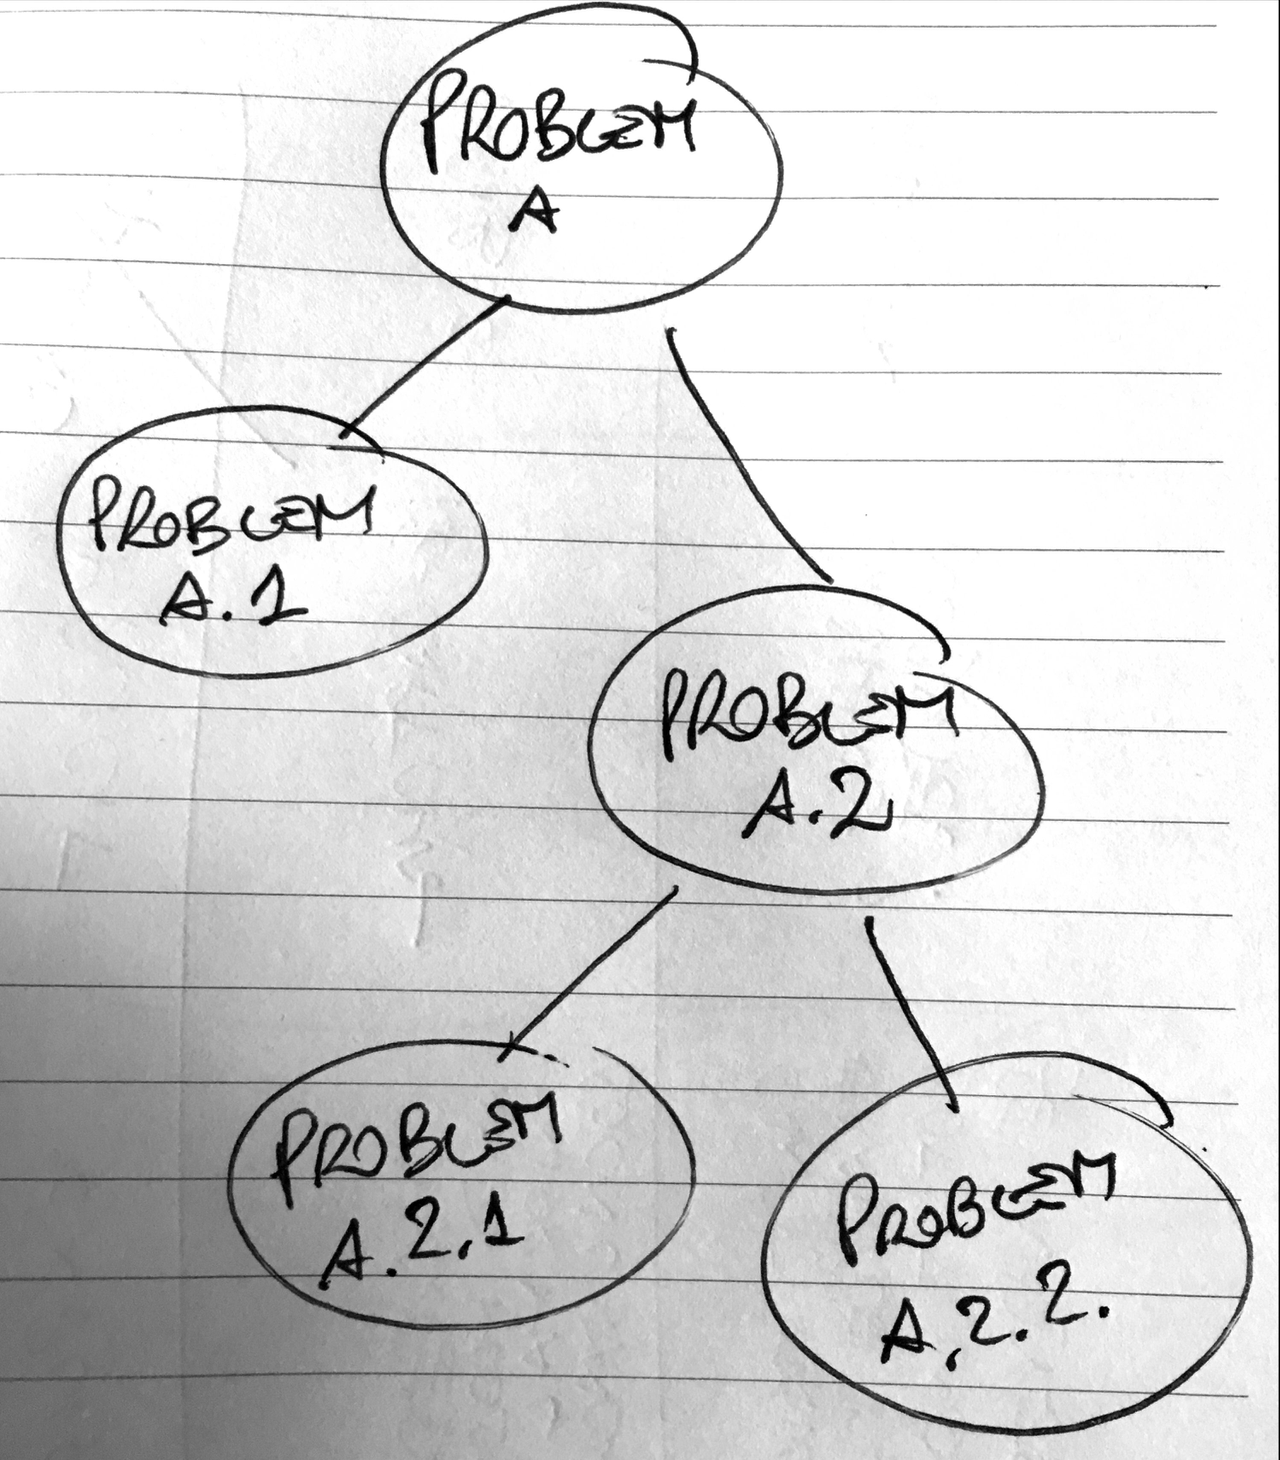
\includegraphics[width=0.95\textwidth]{social-machine-mix-1.png}
    	\caption{This picture should not be here, but apparently it is a nightmare in LaTeX.}
    	\label{fig:social_machine_mix_1}
    \end{figure*}

    For simplicity, only data from authoritative sources is used, such as government bodies, and it is assumed to be of the highest possible quality, equivalent to what could be called {\it ground truth}. It is for this reason that no tasks related to the validation of the open data sources is considered in scope.
    
    The open data available at the moment of writing makes it possible to divide the creation of OLAF in two main sub-problems {\it p1} and {\it p2}. 
    
    \begin{itemize}
        \item {\it p1}: Create a list of all valid house numbers and house names for each road listed in Ordnance Survey's "Open Names"\footnote{SOME REFERENCE}.
        \item {\it p2}: Create a list of the associations between each of the house number and names above and the list of current\footnote{Postcodes can change. The problem of documenting how addresses change postcode in time is relevant but outside of the scope of research.} postcodes listed in Ordnance Survey's "Open Names". 
    \end{itemize}

    Problem {\it p2} is not discussed in this paper. 
    
    Problem {\it p1} can be further decomposed, again thanks to the availability of open data sources:
    
    \begin{itemize}
        \item {\it p1.1}: Collect the list of house numbers and house names for each existing road from citation in Land Registry's "Price Paid"\footnote{SOME REFERENCE}
        \item {\it p1.2}: Statistically infer the existence of house numbers from the house numbers collected above.
        \item {\it p1.3}: Complement and correct the above through surveying.
    \end{itemize}

\subsection{Task model}

    The following is a description of the approach that was used for crowdsourcing addresses, that is common to all experimental conditions that were tested.
    
    \textbf{Requester.} The Requester desires to validate the existence of a series of house numbers (e.g. "3" or "7A") in a specified street. Those were previously inferred algorithmically from the observation of \textit{existing} house numbers, as sourced from published open datasets\footnote{See the GitHub repository at \url{https://github.com/Digital-Contraptions-Imaginarium/OLAF-yr2_reference_data} to learn about the reference open data we used, and the repository at \url{https://github.com/Digital-Contraptions-Imaginarium/OLAF-yr2_inference_data} for the inference algorithms.}. When the pictures in the survey tool are of insufficient quality to be read intelligibly (e.g. a house number could be "7A" but it is not clear) it is useful to the Requester to be informed of that. The Requester requires the help of human agents to carry out the tasks, that we will call Workers in the following.
    
    \textbf{Task.} Each HIT (Human Intelligence Task) consists of verifying the existence in a given street of a given specific tuple of inferred house numbers {[}SOME MATHS SYMBOLS HERE{]} that is a subset of the whole set of inferred house numbers for that street {[}SOME MATHS SYMBOLS HERE{]}. 
    
    \textbf{Strategy.} 
    {[}TO BE WRITTEN, DEPENDS ON THE EXPERIMENT SCENARIOS DEFINITION.{]}
    
    \textbf{Crowd $\rightarrow$ Worker.} Each Worker performs her task by declaring, for each house number in the given tuple and street, if a) it can be found by using the survey tool, b) it can't be found or c) it cannot be said with certainty (e.g. if some of the pictures are blurred and could correspond to the house number being searched). Multiple Workers are asked to validate the same tuple and the resulting data is chosen through majority voting.
    
    \textbf{Reliability.} When collecting data to build a dataset that is intended to be published under an open licence, the option to assess its \textit{quality} by comparison with other sources is often not available, for many reason. An alternative source of the same data could simply not be available. Moreover, from an intellectual property perspective, the comparison could make the former "derivative work" of the latter, hence compromising the purpose{[}SOME REFERENCE OR FOOTNOTE TO PUT MORE MEAT AROUND THIS POINT{]}. 
    
    What is possible, instead, is to estimate the \textit{reliability} of the crowdsourced data, independently of any actual knowledge of other sources and/or the ground truth. 
    
    In OLAF's case, the approach described is considered equivalent to what is used for crowdsourcing the acquisition of labels for data items when the labelling is imperfect, that is extensively covered in literature, e.g. in \cite{sheng2008get} or \cite{Welinder:2010vkb}{[STILL HAVE TO READ THE LATTER{]}. 
    
    The quality of the Workers' contribution could be measured by using gold standard tasks \cite{Oleson:2011tx}, e.g. asking them to validate sets of house numbers whose existence is already known. Because of the elementary complexity of the tasks, though, it was assumed that anything standing between the Worker and the actual required tasks would hinder their contribution in volume and quality and compromise furtherance.
    
    Lacking an assessment of the individual Worker's reliability, the option of preferring the best individual Workers vs using multiple labellers becomes unavailable, hence the need to use majority voting. 
    
    For simplicity, all Workers are considered equivalent from a reliability perspective, and the quality of their individual output assumed $ > 0.5 $, so that the \textit{uniform labeller quality} (see \cite{sheng2008get}) of the data chosen through majority voting increases as the number of labellers is increased.

\subsection{Recruitment}
\subsection{Design}
\subsection{The virtual survey tool}

    Some text before.
    
    \begin{figure*}
    	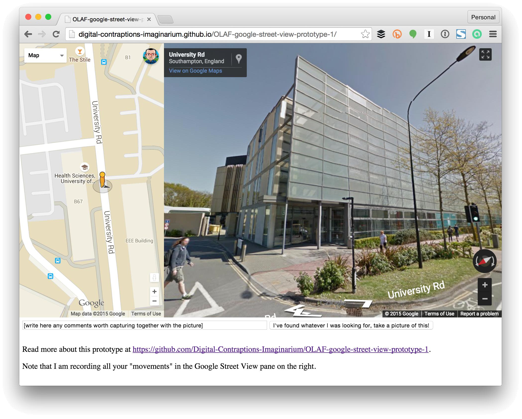
\includegraphics[width=0.95\textwidth]{some_picture.png}
    	\caption{This picture should not be here, but apparently it is a nightmare in LaTeX.}
    	\label{fig:some_figure}
    \end{figure*}
    
    \paragraph{}
    
    Some text after.
	
\subsection{Scalability}

    [THE CALL FOR PAPER EXPLICITLY SAYS THAT "EVIDENCE OF USE IN PRACTICE AND/OR DEMONSTRATION OF SCALABILITY IS REGARDED AS A PLUS"]

\subsection{{[}description of additional conditions to test X{]}}
\subsection{{[}description of additional conditions to test Y{]}}
